\section{Data Description}
\label{sec:Data}

\begin{table}[tb!]
    \centering
    \caption{16 input parameters for the ABC-SMC inference model. As constant parameters such as $K$ and $rrd$ do not affect the simulation results, they are not rendered in our visual designs.}
    \label{tab:input_params}
    \resizebox{\columnwidth}{!}{%
        \begin{tabular}{|l|l|}
            \hline
            \textbf{Name} & \textbf{Description}                                                       \\
            \hline
            \hline
            T\_lat        & Mean latent period (days)                                                  \\
            \hline
            juvp\_s       & Probability of juvenile developing symptoms                                \\
            \hline
            T\_inf        & Mean asymptomatic period (days)                                            \\
            \hline
            T\_rec        & Mean time to recovery if symptomatic (days)                                \\
            \hline
            T\_sym        & Mean symptomatic period prior to hospitalization (days)                    \\
            \hline
            T\_hos        & Mean hospitalization stay (days)                                           \\
            \hline
            inf\_asym     & Reduction factor of infectiousness for asymptomatic infectious individuals \\
            \hline
            p\_inf        & Probability of Infection                                                   \\
            \hline
            p\_hcw        & Probability of Infection (Healthcare Worker)                               \\
            \hline
            c\_hcw        & Mean number of Healthcare Worker contacts per day                          \\
            \hline
            d             & Proportion of population observing social distancing                       \\
            \hline
            q             & Proportion of normal contact made by people self-isolating                 \\
            \hline
            p\_s          & Age-dependent probability of developing symptoms                           \\
            \hline
            rrd           & Risk of death if not hospitalized                                          \\
            \hline
            lambda        & Background transmission rate                                               \\
            \hline
            K             & Hospital bed capacity                                                      \\
            \hline
        \end{tabular}
    }
\end{table}

\begin{table}[tb!]
    \centering
    \caption{13 output parameters from the simulation performed by the ABC-SMC inference model.}
    \label{tab:output_param}
    \resizebox{\columnwidth}{!}{%
        \begin{tabular}{|l|p{9.25cm}|}
            \hline
            \textbf{Name} & \textbf{Description}
            \\
            \hline
            \hline

            iter          & The simulation number.
            \\
            \hline
            day           & The day number.
            \\
            \hline
            age\_group    & The age group of the population.
            \\
            \hline
            S             & Number of susceptible individuals (not infected).                                                           \\
            \hline
            E             & Number of infected individuals but not yet infectious (exposed).                                            \\
            \hline
            E\_t          & Number of exposed individuals and tested positive.                                                          \\
            \hline
            I\_p          & Number of infected and infectious symptomatic individuals but at pre-clinical stage (show yet no symptoms). \\
            \hline
            I\_t          & Number of tested positive individuals that are infectious.                                                  \\
            \hline
            I            & Number of infected and infectious asymptomatic individuals.                                    \\
            \hline
            I\_s         & Number of infected and infectious symptomatic individuals.                                     \\
            \hline
            H             & Number of infected individuals that are hospitalized.                                                       \\
            \hline
            R             & Number of infected individuals that have recovered from the infection.                                      \\
            \hline
            D             & Number of deceased individuals due to the disease.                                                          \\
            \hline
        \end{tabular}%
    }
\end{table}


The data used in our work includes simulation parameters and outcomes from an \ac{ABC-SMC} inference model \cite{toni2008Approximate} developed by a group of modelers from Durham University, the University of Edinburgh, the University of Exeter, the University of Glasgow, and the London School of Hygiene \& Tropical Medicine.
The pandemic data used for the simulation was collected by NHS Scotland during the first wave of the outbreak in Scotland spanning a period of 59 days \cite{2020Covid19}.

\begin{samepage}
The model was built to analyze the pandemic data and infer the parameters of the model that best fit the data.
The model accepts 16 input parameters (see \Cref{tab:input_params}), and a random seed facilitates the generation of 160 distinct sets of configurations for these input parameters.
The model then employs these configurations as the initial input to perform 1,000 simulation iterations. As the outcome of these simulations, 160 sets of predictions are generated, each containing 13 output parameters, as shown in \Cref{tab:output_param}.

\begin{figure}[tb!]
    \centering
    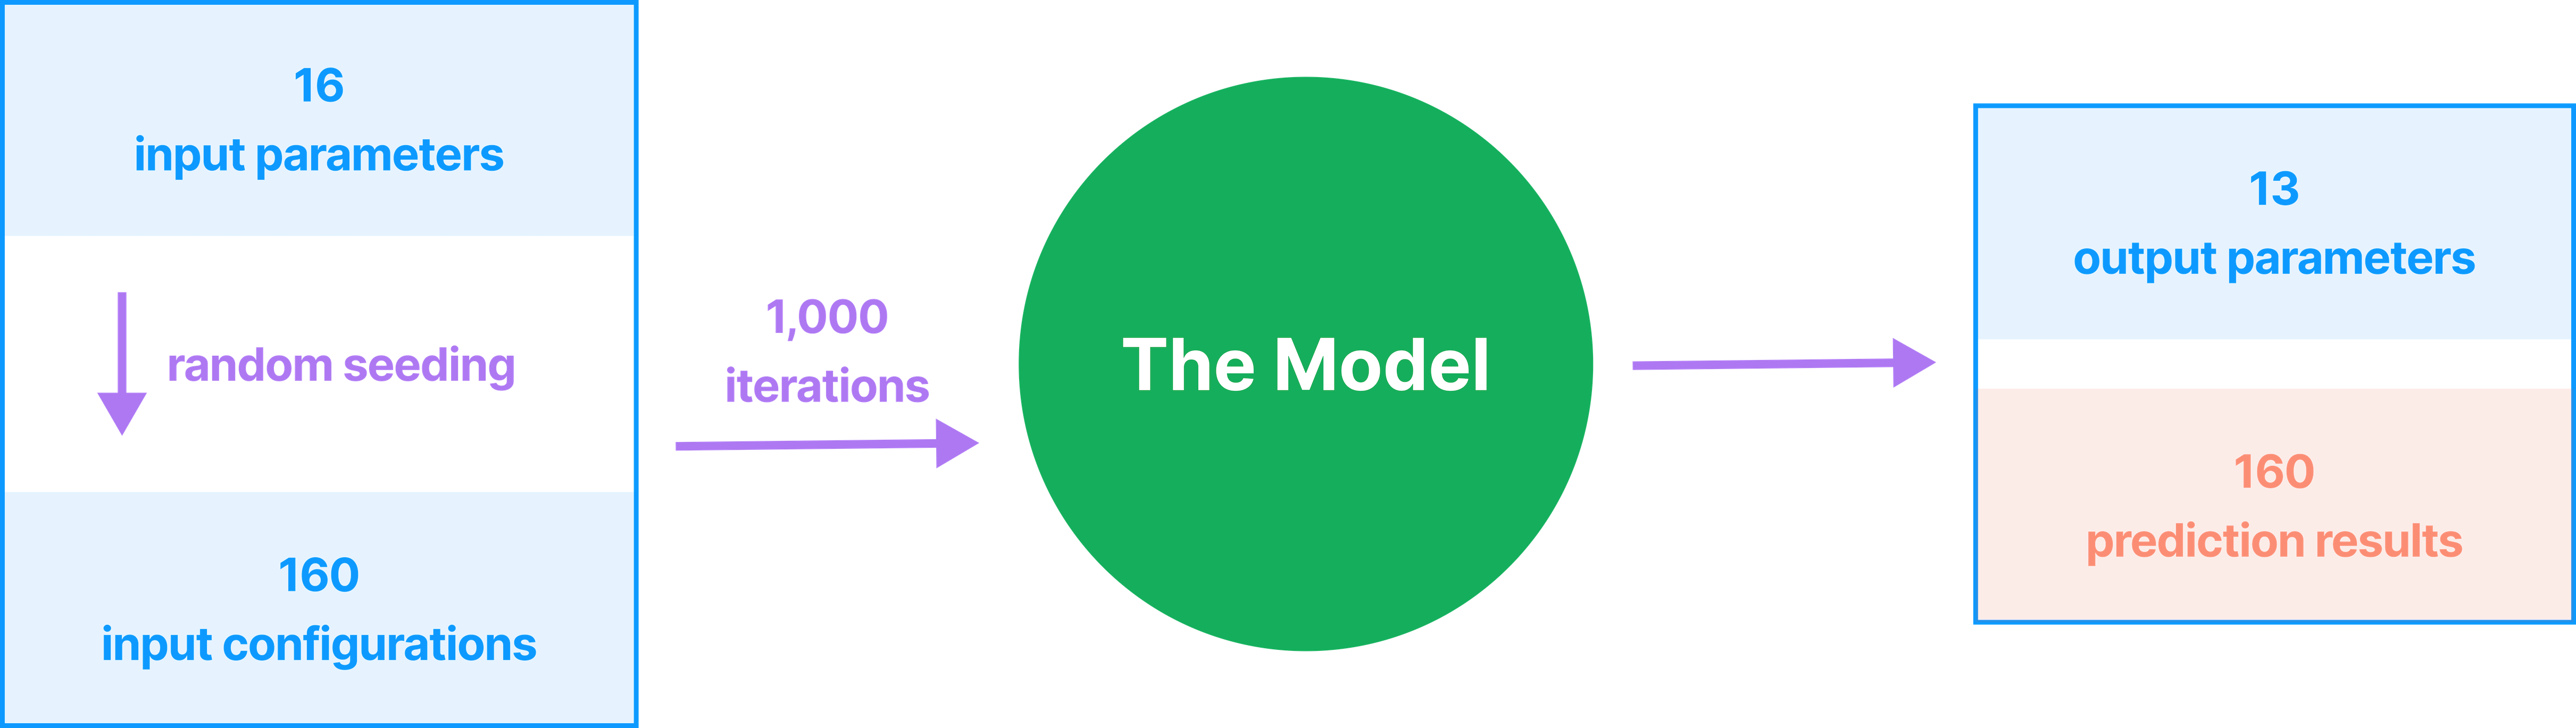
\includegraphics[width=\linewidth]{flow.png}
    \caption{An illustration of the flow from the input parameters to the prediction results. 160 sets of input parameters are used to perform 1,000 simulation iterations, resulting in 160 sets of prediction results.
    }
    \label{fig:flow}
\end{figure}

\end{samepage}



Upon receiving the data, we consulted the modelers to gain insights into the conventional workflow they employ for data processing, as well as the significance and the underlying meaning associated with each input and output parameter. As constant parameters such as $K$ and $rrd$ do not affect the simulation results, they are not rendered in our visual designs.

It is worth mentioning that after plotting the output data using a line chart, an error was immediately spotted, see \Cref{fig:1st-line}, where an unusual spike can be observed on day 20.
The modelers were notified and the bug was fixed.
However, the rectified output file was never made available to us.
